% 等温过程
% 等温过程|体积|压强|状态方程|做功

\pentry{理想气体状态方程\upref{PVnRT}}

等温过程的特征是系统的温度保持不变,即$\mathrm dT=0$.由于理想气体的内能只取决于温度,所以在等温过程中,理想气体的内能也保持不变,也就是说$\mathrm dE=0$.

设想一汽缸壁是绝对不导热的,而底部则是绝对导热的(\autoref{EqTemp_fig1}).现在将气缸的底部和一恒温热源相接触,当活塞上的外界压强无限缓慢地降低时,缸内气体也将随之逐渐膨胀,对外做功气体内能就随之缓慢减少,温度也将随之略微降低.然而,由于气体与恒温热源相接触,当气体温度比热源温度略低时,就有微小的热量传给气体,使气体温度维持原值不变.这一准静态过程就是一个\textbf{等温过程(isothermal process)}.
\begin{figure}[ht]
\centering
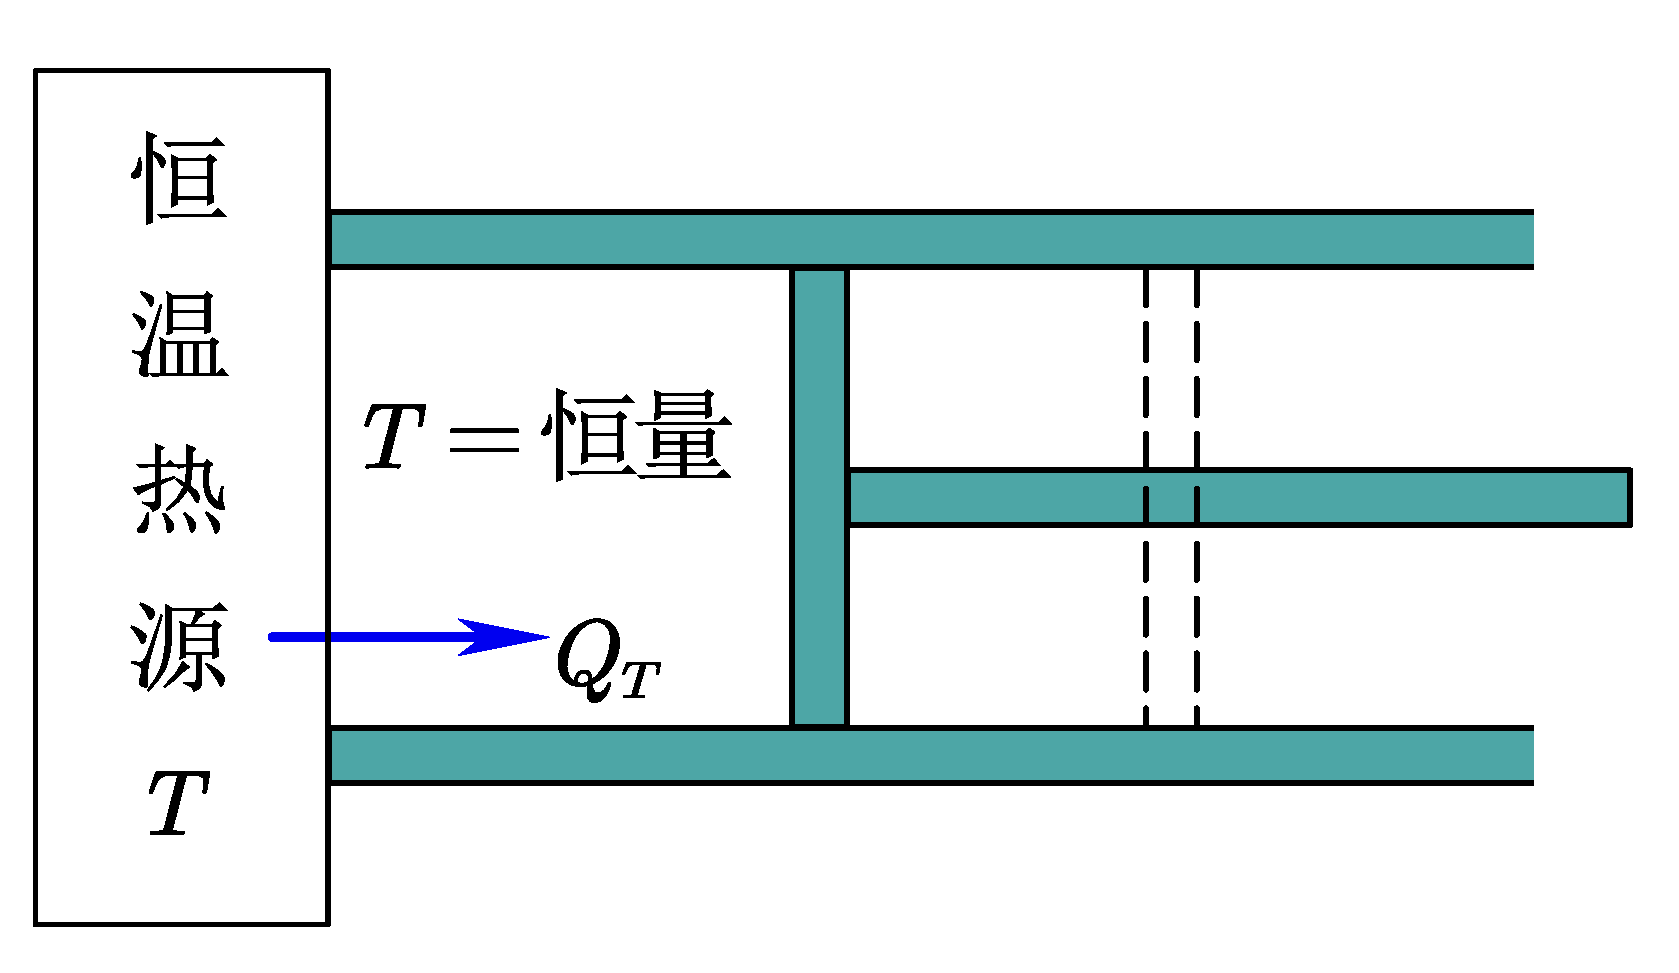
\includegraphics[width=8cm]{./figures/EqTemp_1.pdf}
\caption{气体的等温膨胀} \label{EqTemp_fig1}
\end{figure}

在等温过程中,$p_1V_1=p_2V_2$,系统对外做的功为
\begin{equation}
W= \int_{V_{1}}^{V_{2}} p \mathrm{d} V=\int_{V_{1}}^{V_{2}} \frac{p_{1} V_{1}}{V} \mathrm{d} V=p_{1} V_{1} \ln \frac{V_{2}}{V_{1}}=p_{1} V_{1} \ln \frac{p_{1}}{p_{2}}
\end{equation}

根据理想气体状态方程可得
\begin{equation}
W=\frac{m}{M} R T \ln \frac{V_{2}}{V_{1}}=\frac{m}{M} R T \ln \frac{p_{1}}{p_{2}}
\end{equation}

又根据热力学第一定律,系统在等温过程中所吸收的热量应和它所做的功相等,即
\begin{equation}
Q_{T}=W=\frac{m}{M} R T \ln \frac{V_{2}}{V_{1}}=\frac{m}{M} R T \ln \frac{p_{1}}{p_{2}}
\end{equation}

那么等温过程在$p-V$图上长什么样呢?当然是一条双曲线上的一段.这种双曲线就叫做\textbf{等温线(isotherm)}.如\autoref{EqTemp_fig2} 所示,$\rm I\to II$就是一个等温膨胀过程.在等温膨胀过程中,理想气体所吸取的热量全部转化为对外所做的功;反之,在等温压缩时.外界对理想气体所做的功,将全部转化为传给恒温热源的热量.

\begin{figure}[ht]
\centering
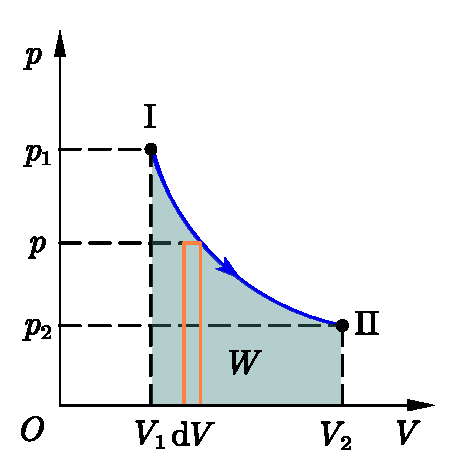
\includegraphics[width=5cm]{./figures/EqTemp_2.pdf}
\caption{等温过程中功的计算} \label{EqTemp_fig2}
\end{figure}
